\documentclass{article}
\usepackage{tikz}
\usepackage{amsmath}

\begin{document}

\begin{figure}[h]
    \centering
    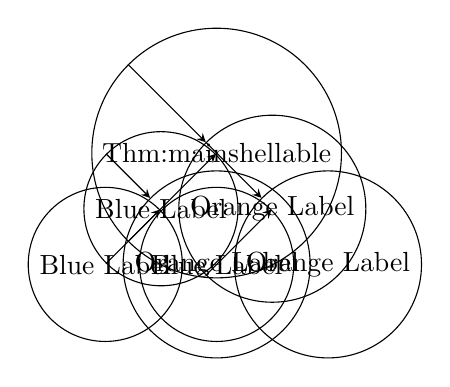
\begin{tikzpicture}[level distance=2cm,
        level 1/.style={sibling distance=4cm},
        level 2/.style={sibling distance=2cm}]
        
        % Nodes
        \node[draw,circle] (root) {Thm:mainshellable};
        \node[draw,circle,below left of=root] (blue1) {Blue Label};
        \node[draw,circle,below right of=root] (orange1) {Orange Label};
        \node[draw,circle,below left of=blue1] (blue2) {Blue Label};
        \node[draw,circle,below right of=blue1] (orange2) {Orange Label};
        \node[draw,circle,below left of=orange1] (blue3) {Blue Label};
        \node[draw,circle,below right of=orange1] (orange3) {Orange Label};
        
        % Edges
        \draw[-stealth] (root) -- (blue1);
        \draw[-stealth] (root) -- (orange1);
        \draw[-stealth] (blue1) -- (blue2);
        \draw[-stealth] (blue1) -- (orange2);
        \draw[-stealth] (orange1) -- (blue3);
        \draw[-stealth] (orange1) -- (orange3);
    \end{tikzpicture}
    
    \caption{Illustration of the Proof of Thm:mainshellable}
    \label{fig:thm_mainshellable}
\end{figure}

% Equations around the figure
\[
\begin{aligned}
    &E_1: \quad \text{Some Equation} \\
    &E_2: \quad \text{Another Equation} \\
    &E_3: \quad \text{Yet Another Equation}
\end{aligned}
\]

\end{document}